%%%%%%%%%%%%%%%%%%%%%%%%%%%%%%%%%%%%%%
\section{Estimation with constrains}
%%%%%%%%%%%%%%%%%%%%%%%%%%%%%%%%%%%%%%


%%%%%%%%%%%%%%%%%%%%%%%%%%%%%%%%%
\subsection{General principles}

Sometimes it may be useful to impose a certain parametric shape on the estimator, $\hat S = f_{\bf w}(\bf X)$, where ${\bf w}$ is a vector containing all the parameters of the function. For example, in a case with two observations ${\bf X} = [X_1, X_2]^T$, it might be a design requirement to restrict the estimator search to the family of quadratic estimators of the form $\hat S = w_0 + w_1 X_1^2 + w_2 X_2^2$. In these cases, the estimator design task is to find the optimal parameter vector ${\bf w}^*$ which provides a minimum average cost subject to the constraint imposed in the estimator architecture:

\begin{align}
{\bf w}^* & = \arg\min_{\bf w}\; \mathbb{E}\{c(S,\hat S)\} = \arg\min_{\bf w} \; \mathbb{E}\{c(S,f_{\bf w}({\bf X}))\} \nonumber\\
 &= \arg\min_{\bf w} \int_{\bf x} \int_s c(s,f_{\bf w}({\bf x})) p_{S,{\bf X}}(s,{\bf x}) ds d{\bf x}
\end{align}

It can easily be understood that the imposition of constraints on the analytical form of the estimator results in incurring a higher average cost than would be obtained using the Bayesian estimator associated with the same cost function\footnote{The only exception to this rule is precisely the case where the constraints imposed allow the optimal estimator to be obtained or, in other words, when the Bayesian estimator presents an analytical form compatible with the constraints imposed.}. However, there may be practical reasons that make the use of the former preferable, for example for simplicity in the design or application of the estimator. An example of this can be found in the Section \ref{sec:est_lineal}, dedicated to the study of linear estimators with minimum mean squared error.

%%%%%%%%%%%%%%%
\begin{example}[{Calculating an Estimator with Constrains}]
\label{CalculoECM_rest}
Continuing the example \ref{CalculoECM2}, we want to calculate the minimum quadratic mean error estimator that has the form $\hat{s} = wx^2$. Starting from the mean cost given the observation calculated in \eqref{Est:ECMsx}, the expression of the global average cost can be obtained as

\begin{equation}
\label{ec:coste_medio2}
\begin{split}
\mathbb{E}\{c(S,\hat S)\} 
   &= \int_{\bf x} \mathbb{E}\{c(S,\hat s)|X=x\} \;p_{\bf X}(\bf x) d{\bf x}  \\
   &= \int_{\bf x} \left(\frac{1}{3}x^2 -\hat{s}x +\hat{s}^2 \right) 
                   p_{\bf X}(\bf x) d{\bf x}
\end{split}
\end{equation}
Forcing $\hat{s} = wx^2$ and taking into account that $p_{\bf X}({\bf x})=1$ for $ 0<x<1$ , you get the global average cost as a function of $w$.
\begin{align}
\mathbb{E}\{c(S,w{\bf X}^2)\} 
   & = \int_{\bf x} \left(\frac{1}{3}x^2 - wx^3 + w^2x^4 \right) d{\bf x} \\
   & = \frac{1}{9} - \frac{1}{4} w + \frac{1}{5} w^2
\label{Est:ECMwx2}
\end{align}
The $w^*$ value that optimizes \eqref{Est:ECMwx2} can be calculated by deriving respect to $w$ and zeroing the expression obtained:
\begin{align}
\left. \frac{d}{d\hat{w}} \mathbb{E}\{c(S,w{\bf X}^2)\} \right|_{w=w^*} 
    &= - \frac{1}{4} + \frac{2}{5} w^* =0,
\end{align}
\begin{equation}
\label{eq:sopt_58}
w^* = \frac{5}{8},
\end{equation}
and therefore the estimator sought is: $\hat{s} = \frac{5}{8}x^2$.

\end{example}\vspace{0.4cm}
%%%%%%%%%%%%%


%%%%%%%%%%%%%%%%%%%%%%%%%%%%%%%%%%%%%%%%%%%%%%%%%%%%%%%%%%%%%%%
\subsection{Linear estimation of minimum squared mean error}
\label{sec:est_lineal}

In this section we will focus on the study of random variable estimators that obtain their output as a linear combination of the values of the observations, using the minimization of the mean squared error as design criterion. Therefore, we will exclusively consider estimators that calculate their output as
\begin{equation}
\hat S = w_0 + w_1 X_1 + \dots + w_N X_N
\end{equation}

where $N$ denotes the number of available observable variables, $\{X_i\}_{i=1}^N$, and $\{w_i\}_{i=0}^{N}$ are the weights that characterize the estimator. In this context, it is common to refer to the term independent of the above expression, $w_0$, as a bias term. For analytical simplicity, it is more convenient to enter the following matrix notation:

\begin{equation}
\hat S = w_0 + {\bf w}^T {\bf X} = {\bf w}_{\text{e}}^T {\bf X}_{\text{e}}
\label{Est:Sestlineal}
\end{equation}
where ${\bf w} = [w_1,\dots,w_N]^T$ and ${\bf X} = [X_1,\dots,X_N]^T$ are the (column) vectors  of parameters and observations, respectively, and ${\bf w}_{\text{e}} = [w_0, {\bf w}^T]^T$ and ${\bf X}_{\text{e}} = [1, {\bf X}^T]^T$ are extended versions of these vectors.

It can be understood that, by imposing a restriction on the analytical form implemented by the estimator, linear estimators will generally obtain lower performance than the optimal Bayesian estimator. However, the interest of linear estimators is justified by their simplicity and ease of design. As we shall see, for the calculation of the linear estimator of minimum squared mean error, it will be sufficient to know the first and second order statistical moments (means and covariances) associated with the observable variables and the variable to be estimated.

%On the other hand, the use of linear estimators is fully justified in certain circumstances, for example when dealing with variables with Gaussian distributions, since, as we saw in the previous section, in this case the Bayesian estimator with the minimum squared mean error has a linear architecture. 


%%%%%%%%%%%%%%%%%%%%%%%%%%%%%%%%%%%%%%%%%%%%%%%%%%%%%%%%%%%%%%%%%%%%%%
\subsubsection{Minimization of the {mean squared error}.}% y ecuaciones normales}

As we have already mentioned, we will consider as design criteria the squared error, $c(e) = (s-\hat s)^2$, so the optimal weight vector will be the one that minimizes the average value of this cost function:

\begin{equation}
{\bf w}_\text{e}^* = \arg\min_{{\bf w}_\text{e}} \; \mathbb{E}\{(S - \hat S)^2\} =  \arg\min_{{\bf w}_\text{e}}\;  \mathbb{E}\{(S - {\bf w}_{\text{e}}^T {\bf X}_{\text{e}})^2\}
\end{equation}
and we will refer to the linear estimator associated with this optimal weight vector as $\hat S_\text{LMSE}$: 
$$\hat S_\text{LMSE} = {{\bf w}_{\text{e}}^*}^T {\bf X}_{\text{e}}$$

%%%%%%%%%%%%%%
\begin{figure}[htb]
  \begin{center}
  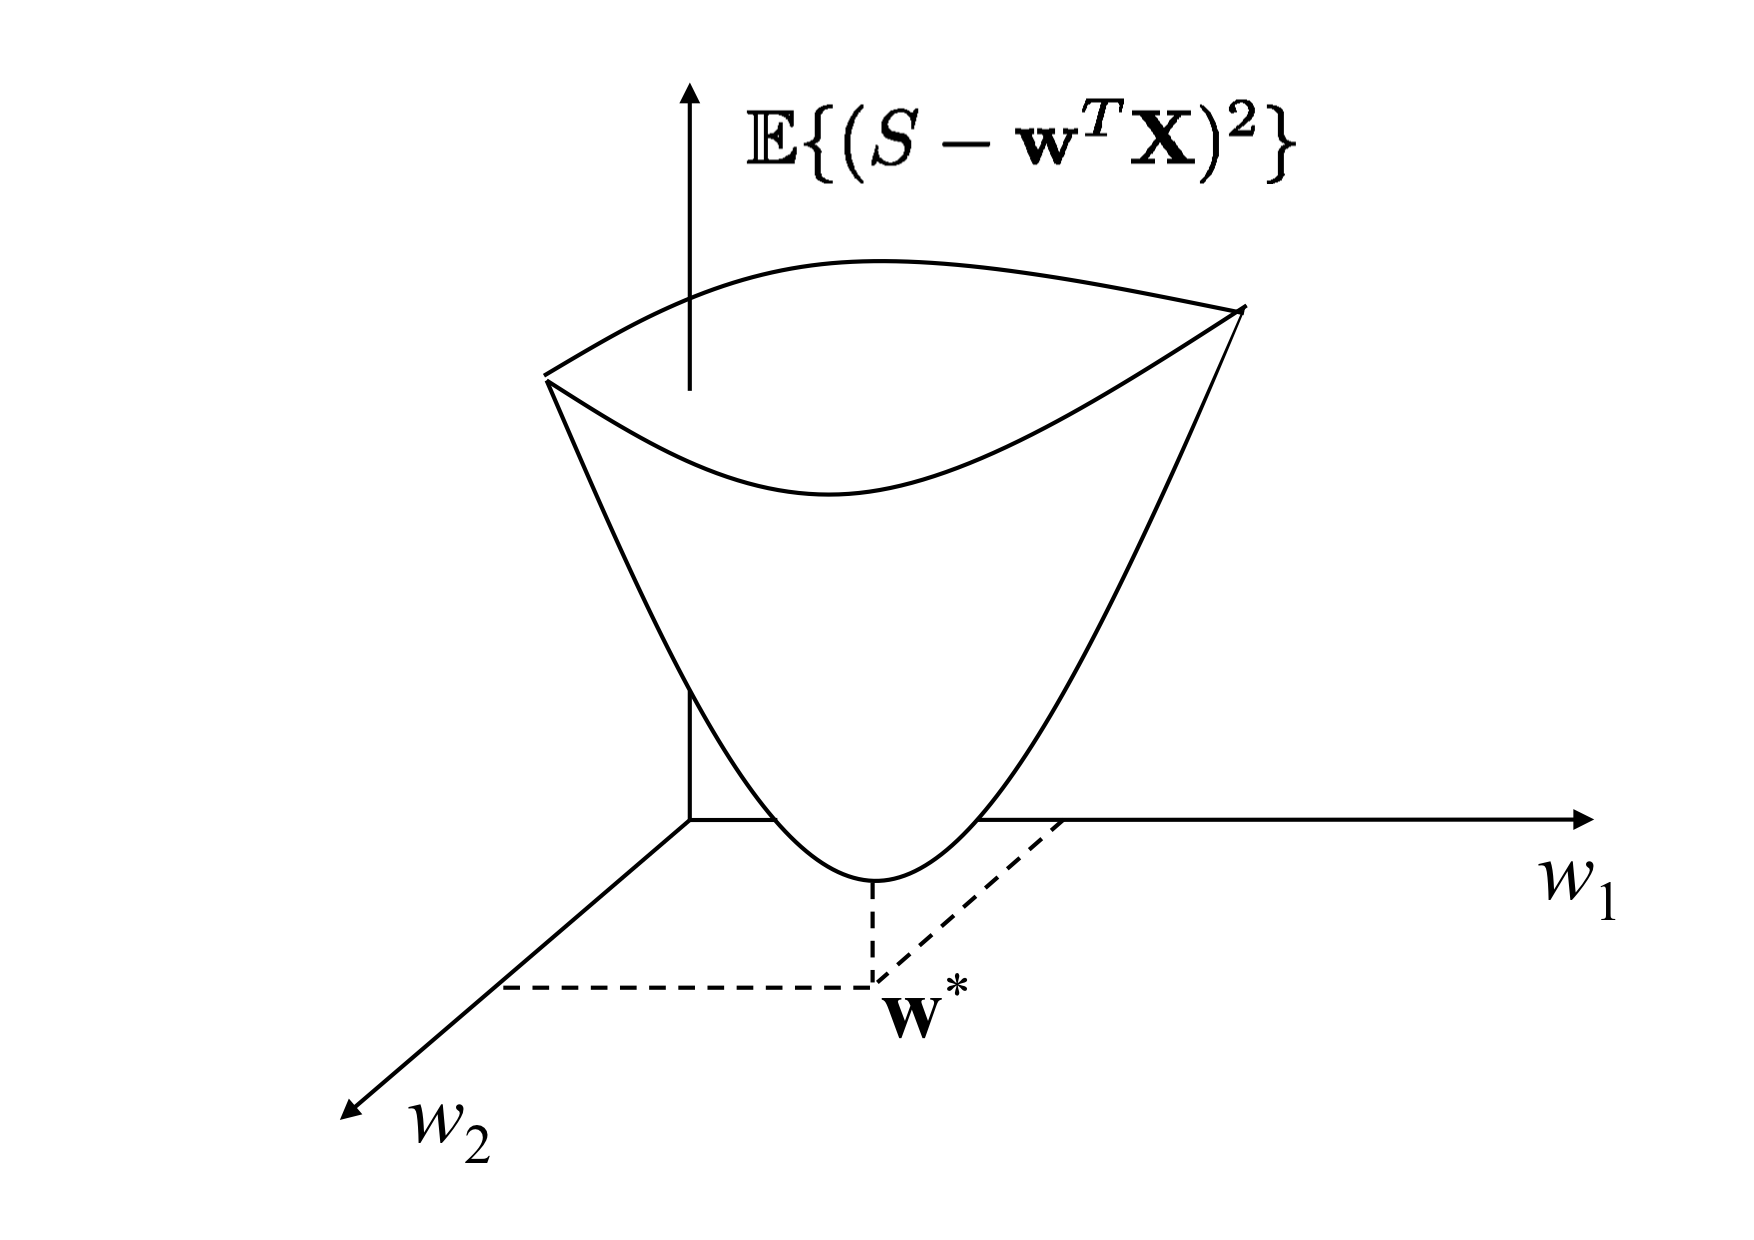
\includegraphics[width=10cm]{Figures//linear_est_error_surface.png}
    \caption{Surface of the mean squared error of the linear estimator as a function of the estimator weights.}
    \label{fig:linear_est_error_surface}
  \end{center}
\end{figure}
%%%%%%%%%%%%

Figure \ref{fig:linear_est_error_surface} represents the error surface in a case with two observations. Being the function to minimize quadratic in weights (minimization argument), the error surface will take the form of a $N$ dimensional paraboloid. In addition, since the average cost is not negative, it is guaranteed that the function is convex, and its minimum can be located by equaling $\bf 0$ the gradient of the average cost with respect to the weight vector\footnote{The gradient of a function scale $f({\bf w})$ with respect to the vector ${\bf w}$ is defined as a vector formed by the derivatives of the function with respect to each one of the components of $\bf w$: $\nabla_{{\bf w}} f({\bf w}) = \left[\frac{\partial f}{\partial w_1}, \dots \frac{\partial f}{\partial w_N}\right]^T$.}:

\begin{equation}
\label{ec:ecs_normales_1}
\begin{split}
\left. \nabla_{{\bf w}_{\text{e}}} \mathbb{E}\{(S - \hat S)^2\} \right|_{{\bf w}_{\text{e}} 
   = {\bf w}_{\text{e}}^*} 
 & = \left. -2 \mathbb{E}\{(S - {\bf w}_{\text{e}}^T {\bf X}_{\text{e}}) {\bf X}_{\text{e}} \} \right|_{{\bf w}_{\text{e}} = {\bf w}_{\text{e}}^*} = \\
 & = -2 \mathbb{E}\{(S -  {{\bf w}_{\text{e}}^*}^T {\bf X}_{\text{e}}) {\bf X}_{\text{e}} \} = {\bf 0}
\end{split}
\end{equation}

The second line of the above expression defines the conditions to be met by the optimal weight vector. Note that this equation is actually a system of $N+1$ equations (as many as dimensions have ${\bf X}_{\text{e}}$) with $N+1$ unknowns (the components of ${\bf w}_{\text{e}^*}$).

In order to find the optimal {weight} vector, it is convenient to rewrite the last line of \eqref{ec:ecs_normales_1} as follows 

\begin{equation}
\mathbb{E}\{S {\bf X}_{\text{e}} \}
    = \mathbb{E}\{ {\bf X}_\text{e} ({\bf X}_{\text{e}}^T {\bf w}_{\text{e}}^*)  \}
\label{Est:EcDelELv}
\end{equation}
Defining the cross-correlation vector
\begin{equation}
{\bf r}_{S{\bf X}_e} = \mathbb{E}\{S{\bf X}_e\}
\end{equation}
and the correlation matrix 
\begin{equation}
{{\bf R}_{{\bf X}_e}} = \mathbb{E}\{{\bf X}_e{\bf X}_e^T\}
\end{equation}
(which is a symmetrical matrix) ec. \eqref{Est:EcDelELv} can be written as
\begin{equation}
\label{Est.ec:RxWr}
{\bf r}_{S{\bf X}_e} = {{\bf R}_{{\bf X}_e}} {\bf w}_{\text{e}}^* 
\end{equation}
Thus, the searched weight vector is:
\begin{framed}
\begin{equation}
\label{Est.ec:weopt}
 {\bf w}_{\text{e}}^* = {{\bf R}_{{\bf X}_e}^{-1}} {\bf r}_{S{\bf X}_e} 
\end{equation}
\end{framed}



%%%%%%%%%%%%%%%%%%%%%%%%%%%%%%%%%%%%%%%%%%%%%%%%%%%%%%%
\subsubsection{Properties of the optimal linear estimator}

Equation \eqref{Est.ec:RxWr} solves the problem of calculating the weights of the estimator $\hat S_\text{LMSE}$. But it is interesting to return to the vector equation  \eqref{ec:ecs_normales_1} to analyze some of its properties. Note that the term in parentheses in this equation is the estimation error
\begin{equation}
E^* = S - {{\bf w}_{\text{e}}^*}^T {\bf X}_{\text{e}}
\end{equation}
so we can rewrite \eqref{ec:ecs_normales_1} as
\begin{equation}
\label{Est:SLMSinsesgado0}
\mathbb{E}\{E^* {\bf X}_{\text{e}})\} = {\bf 0}
\end{equation}
Taking, on the one hand, the first component of this equation (taking into account that $X_{\text{e},1}=1$, and the rest on the other hand, two fundamental properties of the lowest quadratic mean error linear estimator are obtained:
\begin{description}
\item[{\bf Property 1:}] The error has zero mean:
\begin{equation}
\label{Est:SLMSinsesgado}
\mathbb{E}\{E^*\} = {\bf 0}
\end{equation}
When an estimator has this property it is said that it is {\bf unbiased}.% {Volveremos sobre esta propiedad en la sec. \ref{Est:Sec:CaracterEstim}.}
\item [{\bf Property 2 (Orthogonality Principle):}] the error is statistically orthogonal to the observations:
\begin{equation}
\label{Est:PrincipioOrtV1}
\mathbb{E}\{E^* {\bf X}\} = {\bf 0}
\end{equation}
\end{description}



%%%%%%%%%%%%%%%%%%%%%%%%%%%%%%%%%%%%%%%%%%%%%%%%%%%%%%%%%%%%%%%%%%
\subsubsection{{Alternative expression of the estimator}}
Expanding Ecs. \eqref{Est:SLMSinsesgado} and \eqref{Est:PrincipioOrtV1}, we can obtain the following explicit formulas for the coefficients $w_0^*$ and ${\bf w}^*$ of the estimator:

\begin{framed}
\begin{equation}
w_0^* = m_S - {{\bf w}^*}^T{\bf m_x} 
\label{ec:solucionw0}
\end{equation}
\begin{equation}
\label{ec:solucionw}
{\bf w}^* = {{\bf V}_{\bf X}^{-1}} \; {\bf v}_{S,{\bf X}}\end{equation}
\end{framed}

It can be observed that the role of the bias term $w_0$ is to compensate for differences between the means of the variable to be estimated and the observations. Therefore, when all the variables involved have null means, $w_0^* = 0$. In contrast to the paper of $w_0$, we can affirm that the weight vector ${\bf w}$ minimizes the mean quadratic error of the fluctuations of $S$ around its mean, exploiting for it the existing statistical relation between $S$ and $\bf X$.

We will dedicate this section to obtaining the expressions \eqref{ec:solucionw0} and \eqref{ec:solucionw}. The first is a direct consequence of \eqref{Est:SLMSinsesgado} that can be developed as 

\begin{equation}
m_S - {{\bf w}^*}^T{\bf m_x} - w_0^* =0 
\end{equation}
solving for $w_0^*$, we obtain \eqref{ec:solucionw0}.

{We will now search for an expression for ${\bf w}^*$. From \eqref{Est:PrincipioOrtV1} results
\begin{equation}
\label{Est:PrincipioOrtV2}
\mathbb{E}\{(S - {{{\bf w}^*}^T} {\bf X} - w_0^*) {\bf X}\} = {\bf 0}
\end{equation}
which can be rewritten as
\begin{align}
\label{Est:PrincipioOrtV2b}
\mathbb{E}\{S {\bf X}\} 
   &= \mathbb{E}\{({{\bf w}^*}^T {\bf X} + {w_0^*}) {\bf X}\}     \nonumber\\
   &= \mathbb{E}\{{\bf X} ({{\bf X}^T{\bf w}^*}) \} {+ w_0^*} \mathbb{E}\{{\bf X} \}  \nonumber\\
   &= \mathbb{E}\{{\bf X} {\bf X}^T \}{\bf w}^* + w_0^* {\bf m_X}  
\end{align}
}
Now using the expressions that relate the correlation and covariance of two variables:
\begin{equation}
\mathbb{E}\{S {\bf X}\} = {\bf v}_{S,{\bf X}} + m_S {\bf m_X}
\end{equation}
\begin{equation}
\mathbb{E}\{{\bf X}{\bf X}^T\} = {\bf V_X} + {\bf m_X}{\bf m}_{\bf X}^T
\end{equation}
eq. \eqref{Est:PrincipioOrtV2b} becomes 
\begin{align}
\label{Est:PrincipioOrtV3}
{\bf v}_{S,{\bf X}}  
   &= {\bf V_X}{\bf w}^* + {\bf m_X}{\bf m}_{\bf X}^T{\bf w}^* + w_0^* {\bf m_X} - m_S {\bf m_X}  \nonumber\\ 
   &= {\bf V_X}{\bf w}^* 
    + {\bf m_X}(w_0^* + {\bf m}_{\bf X}^T{\bf w}^* - m_S) 
     \nonumber\\ 
   &= {\bf V_X}{\bf w}^* 
\end{align}
where, in the last equality, we have applied \eqref{ec:solucionw0}. So, solving for ${\bf w}^*$, we get \eqref{ec:solucionw}.



%%%%%%%%%%%%%%%%%%%%%%%%%%%%%%%%%%%%%%%%%%%%%%%%%%%%%%%%%%%%
\subsubsection{Minimum squared mean error}

Here we will calculate the mean squared error associated with the linear estimator of minimum mean squared error, $\hat S_\text{LMSE}$. As commented at the beginning of this section, the mean squared  error obtained will, in general, be higher than the minimum mean squared error of the Bayesian estimator ($\hat S_\text{MMSE}$), except when this last estimator has precisely a linear structure (in this case, it would be the same).

To calculate the mean squared error we only have to develop the expression of the mean quadratic error, particularizing it for $\hat S_\text{LMSE}$ and leaving the result in function of the mathematical expectations of the involved random variables:

\begin{align}
\mathbb{E}\{(S - \hat S_\text{LMSE})^2\} 
   & = \mathbb{E}\{E^*(S - w_0^* - {{\bf w}^*}^T {\bf X})\} \nonumber\\ 
   & = \mathbb{E}\{E^* S\} 
     - w_0^* \mathbb{E}\{E^*\} 
     - {{\bf w}^*}^T \mathbb{E}\{{\bf X}E^*\}  \nonumber\\
   & = \mathbb{E}\{E^* S\} 
\end{align}

where, in the last equality, we have applied the two properties of the minimum quadratic mean error estimator obtained in \eqref{Est:SLMSinsesgado} and \eqref{Est:PrincipioOrtV1}. Operating again the error term, $E^*$, results in
\begin{align}
\mathbb{E}\{(S - \hat S_\text{LMSE})^2\} 
   & = \mathbb{E}\{S (S - w_0^* - {{\bf w}^*}^T {\bf X})\}  \nonumber\\
   & = \mathbb{E}\{S^2\} 
     - w_0^* m_S 
     - {{\bf w}^*}^T ({\bf v}_{S{\bf X}} + m_S {\bf m}_{\bf X})\} \nonumber\\
   & = \mathbb{E}\{S^2\} - m_S (w_0^* {+} {{\bf w}^*}^T {\bf m}_{\bf X})
     - {{\bf w}^*}^T {\bf v}_{S{\bf X}}  \nonumber\\
   & = v_S - {{\bf w}^*}^T {\bf v}_{S{\bf X}} 
\end{align}
%\begin{equation}
%\begin{split}
%\mathbb{E}\{(S - \hat S_\text{LMSE})^2\} 
%   & = \mathbb{E}\{(S - w_0^* - {{\bf w}^*}^T {\bf X})^2\} \\ 
%   & = \mathbb{E}\{S^2\} + {w_0^*}^2 + {{\bf w}^*}^T \mathbb{E}\{{\bf X}{\bf X}^T\}{{\bf w}^*} - 2 w_0^* \mathbb{E}\{S\} \\ 
%& \;\;\;\;\;\; - 2 {{\bf w}^*}^T \mathbb{E}\{S {\bf X}\} - 2 w_0^* {{\bf w}^*}^T \mathbb{E}\{{\bf X}\}
%\end{split}
%\end{equation}
%
%Si introducimos en esta expresión los valores de los pesos óptimos [Ecs. \eqref{ec:solucionw} y \eqref{ec:solucionw0}], y tenemos también en cuenta que $\mathbb{E}\{S^2\} = v_S + \mathbb{E}^2\{S\}$, así como las expresiones análogas para $\mathbb{E}\{S {\bf X}\}$ y $\mathbb{E}\{{\bf X}{\bf X}^T\}$, se puede demostrar que
%\begin{equation}\label{ec:err_LMSE}
%\mathbb{E}\{(S - \hat S_\text{LMSE})^2\} 
%    = v_S - {\bf v}_{S,{\bf X}}^T \; {{\bf V}_{\bf X}^{-1}} \; {\bf v}_{S,{\bf X}}
%\end{equation}
%\end{example}\vspace{0.4cm}

%\begin{exercise}[Cálculo del error cuadrático medio para variables con medias nulas]
%Demuestre el resultado \eqref{ec:err_LMSE} para el caso concreto en que $\mathbb{E}\{S\} = 0$ y $\mathbb{E}\{{\bf X}\} = {\bf 0}.$
%\end{exercise}

%%%%%%%%%%%%%%%%
\begin{exercise}[Linear estimation of minimum mean squared error]
We want to construct a linear estimator of minimum mean squared error that will allow us to estimate the random variable $S$ from the random variables $X_1$ and $X_2$. Knowing that
\begin{equation}
\begin{array}{lll} \mathbb{E}\{S\} = 1/2 & \mathbb{E}\{X_1\} = 1 & \mathbb{E}\{X_2\} = 0 \\ \mathbb{E}\{S^2\} = 4 & \mathbb{E}\{X_1^2\} = 3/2 & \mathbb{E}\{X_2^2\} = 2 \\ \mathbb{E}\{S X_1\} = 1 \;\;\;\;& \mathbb{E}\{S X_2\} = 2 \;\;\;\; & \mathbb{E}\{X_1 X_2\} = 1/2 \end{array}\nonumber
\end{equation}
get the weights from the desired estimator and calculate its squared mean error. Calculate the estimated value for the observation vector: $[X_1,X_2] = [3, 1]$.
\end{exercise}
%%%%%%%%%%%%%%